\section{Multivariable Differential Calculus}

Here are examples related to differential calculus in more than one variable.

\subsection{Envelopes}

In the simplist cases, the \textbf{envelope} of a family \(\mathfrak F\) of curves is a curve \(\gamma\) that is in some sense extremal to the entire family of curves. 
What is often the case, is that every point of the curve \(\gamma\) touches exaclty one curve from the the family \(\mathfrak F\), and furthermore this touching is only tangential (i.e. they cross at an angle of zero). 
This is best illustrated with examples. 

\subsubsection{The Hyperbola as an Envelope}

\subsubsection*{The Set Up}

Consider the family \(\mathfrak F\) of straight lines in \(\mathbb R^2\), where each line crosses the x-axis and y-axis at pairs of points of the form \((s,0)\) and \((0, 1/s)\) for some \(s > 0\). 
So we see that each line is of the form \(\frac{1}{s} x + s y = 1\) for some \(s > 0\).
Some of the lines from the family are pictured in the following figure.

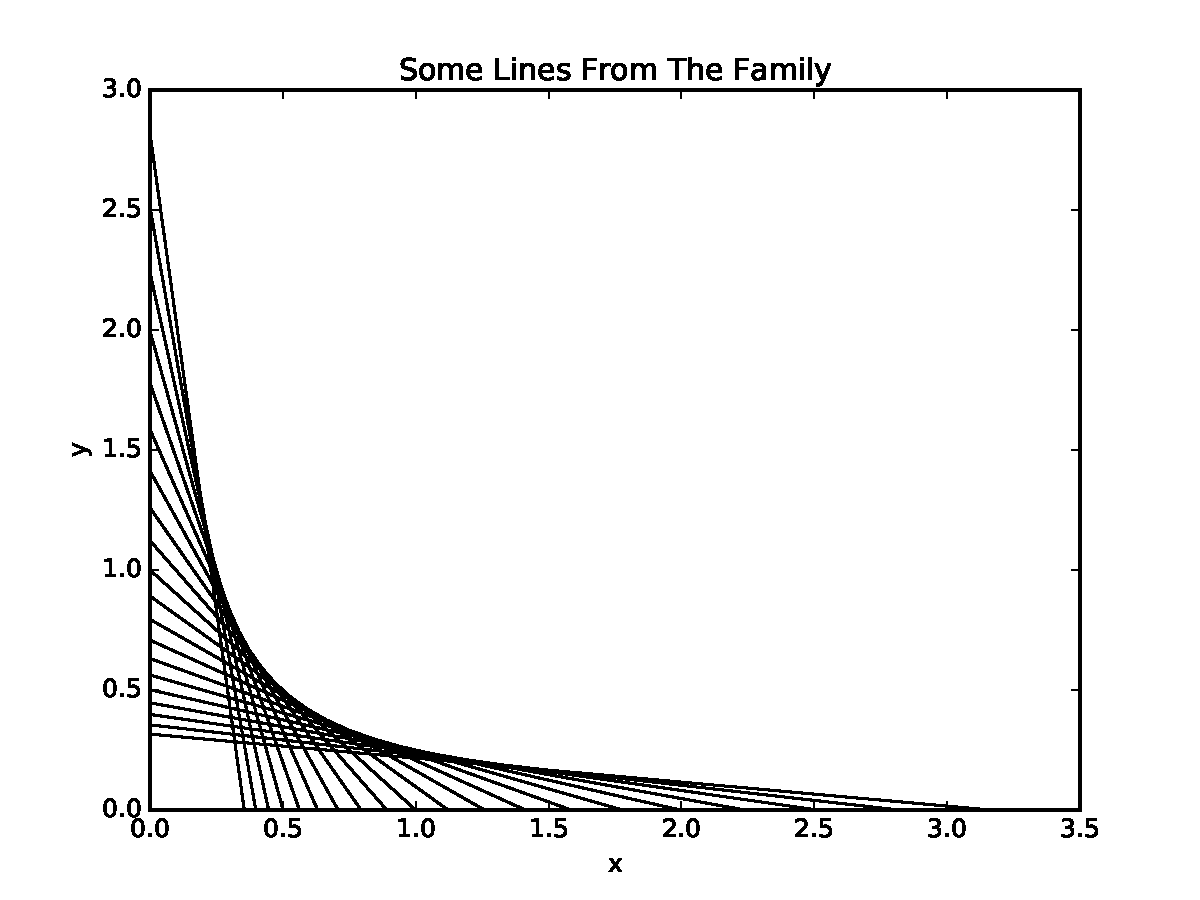
\includegraphics[width = 4.0in]{multiVarDiffCalc/hyperbolaFamily.pdf}

We can see that extemal to the family of lines is a curve concave up in the first quadrant \(\{x, y > 0\}\). In the following figure, you can see the curve superimposed with some of the lines from the family.

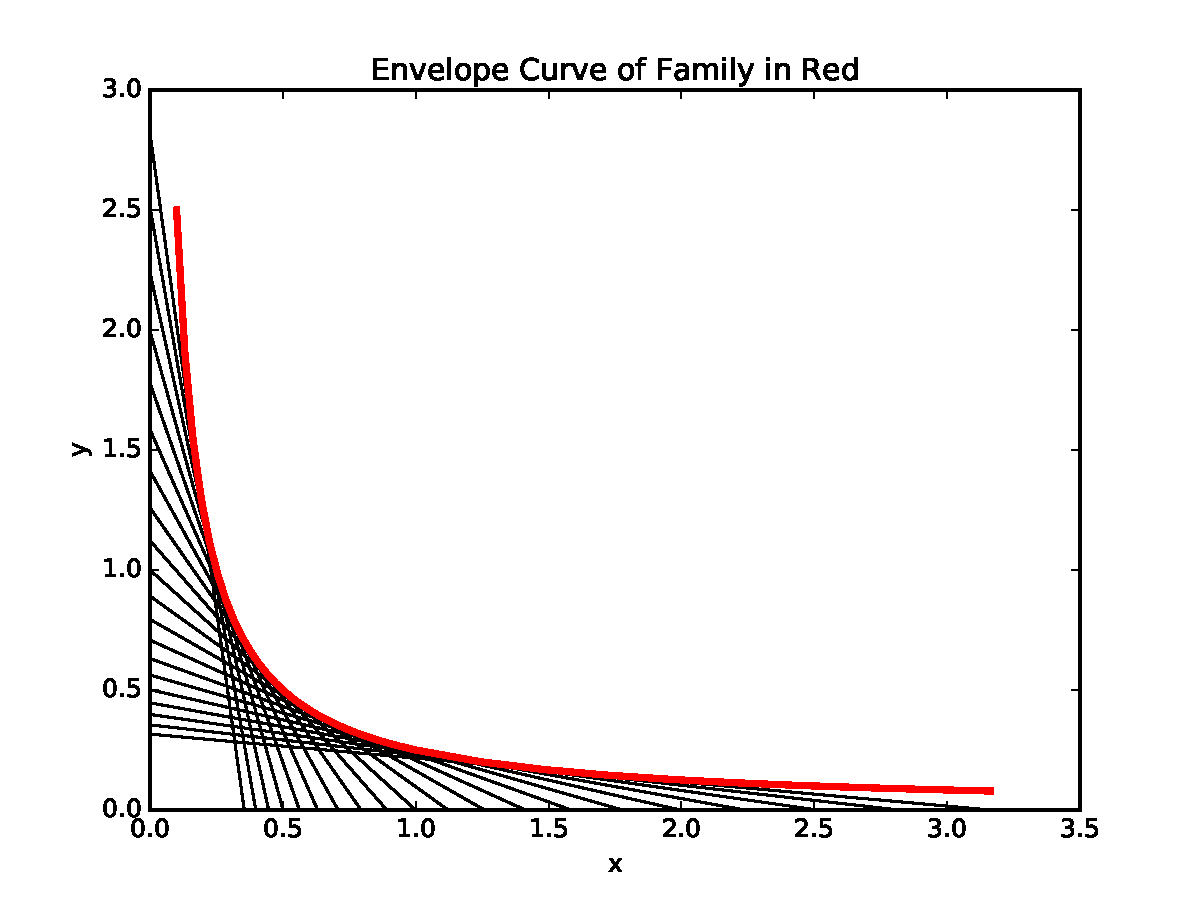
\includegraphics[width = 4.0in]{multiVarDiffCalc/hyperbolaEnvelope.pdf}

\subsubsection*{The Problem}
Let us consider computing the envelope curve \(\gamma(x)\) of the family \(\mathfrak F\). 

\subsubsection*{The Solution}

To compute the envelope curve \(\gamma(x)\), let us consider the auxilliary function
\(g(x,y,s) = \frac{1}{s} x + s y - 1\). Let us see how the Implicit Function Theorem of vector calculus let's us
use \(g(x,y, s)\) to find the exremal envelope curve \(\gamma(x)\). As we discuss this, please consider the similarities to the ordinary first derivative test.

First, consider any point \((x_0, y_0)\) NOT on the extremal envelope curve \(\gamma(x)\), but is touched by some line in \(\mathfrak F\). 
So there is some \(s_0 > 0\) such that \(\frac{1}{s_0} x_0 + s_0 y_0 = 1\); note that this is equivalent to \(g(x_0, y_0, s_0) = 0\). 
Since \((x_0, y_0)\) isn't on the boundary of the region of points touched by lines in \(\mathfrak F\), we know that for any other points \((x_1, y_1)\) close to \((x_0, y_0)\) we may find another line in \(\mathfrak F\) touching \((x_1, y_1)\). 
That is, for every \((x_1, y_1)\) close to \((x_0, y_0)\), we may find \(s_1 > 0\) such that \(g(x_1, y_1, s_1) = 0\).  

This can be summarized as saying that for all points \((x_0, y_0)\) that are touched by a line in \(\mathfrak F\) and also isn't on the envelope \(\gamma\), we can locally solve \(s = S(x,y)\) such that \(g(x, y, S(x, y)) = 0\). Now, you may begin to see the connection to the Implicit Function Theorem.

Recall that the Implicit Function Theorem can only confirm that we CAN locally solve \(s = S(x,y)\) such that \(g(x, y, S(x, y)) = 0\). However, we seek for the extremal points where we CAN'T locally solve. This is similar to the first derivative test of ordinary calculus. Technically, the first derivate test only says when a point is NOT an extemum of a function; then the candidate points for extrema are reduced to some finite list by solving for the vanishing of the derivative.

Here, we are in a similar situation. We solve for a set of candidate points that must contain our extremal curve \(\gamma\). 
It will happen to be the case that our candidate set will allow only one curve and so this must be the envelope.
However, we are being a little reckless here as we haven't proven the curve must exist; we will consider the picture to be very convincing and ignore this technical detail. 

So we seek for when we can't locally solve \(s = S(x,y)\) such that \(g(x, y, S(x, y)) = 0\). The Implicit Function Theorem tells us this will only be possible for those \((x,y,s)\) with \(g(x,y,s) = 0\) and \(\frac{\partial g}{\partial s} (x, y, s) = 0\).

So we look for
\begin{align}
0 & = \frac{\partial g}{\partial s}, \\
&  = -\frac{x}{s^2} + y
\end{align}

We wish to find an equation restricting \(x\) and \(y\); so it is most efficient to solve the above for \(s\). 
Also, from the picture it is clear that we should restrict to \(x, y > 0\). 
Therefore, for \(x, y > 0\), we have \(s = \sqrt{\frac{x}{y}}\). Plugging this into the equation for \(g(x, y, s) = 0\), we get 
\begin{equation}
\sqrt{xy} + \sqrt{xy} - 1 = 0.
\end{equation} 

Therefore, we find that the envelope curve must lie inside the set \(S = \{xy = \frac{1}{4}\}\). However, one will recognize that for each point \(x > 0\), there is only one \(y\) such that \(y \in S\). Therefore, the envelope must be this curve.

So the envelope \(\gamma(x)\) is the curve \(y = \frac{1}{4x}\) for \(x > 0\).  

\subsubsection*{Final Remark}

Note that the set \(S\) is actually a hyperbola. Therefore, the hyperbola can be realized as the envelope of a simple family of straight lines. For this reason, hyperbolas are (approximately) reproducible in "string art": art formed from
straight line segments where each segment is made by tightened string.

\subsection{Differentiable Function With Bounded Non-Continuous Derivatives}

\subsubsection*{Setup}

Functions that are differentiable everywhere do not necessarily have continuous derivatives, even if the derivatives of the function are bounded. For the case of one variable, a classic example is
\begin{equation}
f(x) = \begin{cases}
    x^2 \sin(\frac{1}{x}) & x\neq 0,\\
    0 & x = 0.
    \end{cases}
\end{equation}
Here, the altering of the amplitude by the factor of \(x^2\) forces the function to be differentiable at \(x = 0\) and \(f'(0) = 0\). This can be checked by directly applying the definition of differentiability. However, the derivative \(f'(x)\) alternates infinitely between values close to \(f' = -1\) and \(f' = 1\) as \(x \to 0\). Therefore, the function does not have continuous derivatives.

However, one may wonder if this "infinite frequency oscillation" is necessary. In this example, we show that this is unnecessary in two-dimensions. That is, we construct a function \(u(x,y)\) that is 
differentiable everywhere, has bounded derivatives, and does not have continuous derivatives at \((0,0)\).

\subsubsection*{The Problem}

Find a simple function \(u(x,y)\) such that \(u\) is differentiable on \(\mathbb R^2\), the derivatives of \(u\) are bounded, and at least one of the derivatives of \(u\) is NOT continuous at \((0,0)\).

\subsubsection*{The Solution}

First let us consider a phenomenon in one-variable calculus. If \(g(x)\) is a differentiable function with bounded derivatives: \(|g'| \leq M\), then for any constant \(\lambda > 0\) the function
\(h(x) = \lambda g\left(\frac{x}{\lambda}\right)\) has the same bound for its derivatives, i.e. \(|h'| \leq M\). This is easily proved using the chain rule:
\begin{align}
h'(x) & = \lambda \frac{d}{dx} \left( g\left(\frac{x}{\lambda}\right)\right), \\
    & = \lambda g'\left(\frac{x}{\lambda}\right) \frac{1}{\lambda}, \\
    & = g'\left(\frac{x}{\lambda}\right). 
\end{align}
Therefore, if \(|g'| \leq M\), then \(|h'| \leq M\) too. 

So the idea is that we can construct a function \(u(x,y)\) by setting \(u(x,y) = (x^2 + y^2) h\left(\frac{x}{x^2 + y^2}\right)\) for an appropriate function \(h(x)\). What properties should we require
of \(h(x)\)? First, let's check what is necessary for bounded derivates. Although we were guided by our idea in one-variable differentiation, we must now explicitly check that everything works out okay
since our factor \(x^2 + y^2\) isn't actually constant. 

First, let's calculate the \(x\)-derivative when \((x,y) \neq (0, 0)\):
\begin{align}
\frac{\partial u}{\partial x} & = 2x h + (x^2 + y^2) h' \left(\frac{1}{x^2 + y^2} - \frac{2x^2}{(x^2 + y^2)^2}\right), \\
    & = 2xh + h' - h' \frac{x^2}{x^2 + y^2}. 
\end{align}

Now, let's calculate the \(y\)-derivative when \((x,y) \neq (0,0)\):
\begin{align}
\frac{\partial u}{\partial y} & = 2yh + (x^2 + y^2) h' \frac{2xy}{(x^2 + y^2)^2}, \\
    & = 2yh + h'\frac{2xy}{x^2 + y^2}.
\end{align}

Therefore, we see that the derivatives \(u_x\) and \(u_y\) will be bounded for \((x,y) \neq (0,0)\) when the function \(h(x)\) and its derivative \(h'(x)\) are both bounded; note that expressions like
\(\frac{x^2}{x^2 + y^2}\) and \(\frac{2xy}{x^2 + y^2}\) are bounded for points away from the origin because they are invariant under scaling (i.e. homogeneous of order 0).

Finally, when \(h(x)\) is bounded, the fact that we mulitply \(h\) by \(x^2 + y^2\) to construct \(u\) implies that \(u\) will be differentiable at the origin and that \(u_x(0,0) = u_y(0,0) = 0\).
Now, focus on the expression \(h' \frac{2x^2}{x^2 + y^2}\) in the expression for \(u_x\). If we approach the origin along \(y^4 = x\), then
\begin{align}
h'\left(\frac{x}{x^2 + y^2}\right) & = h'\left(\frac{\sqrt{x}}{x^{3/2} + 1}\right) ,\\
    & \to h'(0).
\end{align} 
Furthermore as we approach the origin along \(y^4 = x\), 
\begin{align}
\frac{x^2}{x^2 + y^2} & = \frac{x^{3/2}}{x^{3/2} + 1}, \\
    & \to 0. 
\end{align}
Therefore, as we approach the origin along \(y^4 = x\), we have that \(u_x \to h'(0)\). So we will want \(h'(0) \neq 0\), e.g. \(h'(0) = 1\).

Let us recap our requirements for \(h(x)\).
\begin{itemize}
\item The function \(h(x)\) is differentiable with continuous derivatives on \(\mathbb R\)
\item The values of the function \(h(x)\) and its derivative \(h'(x)\) are both bounded.
\item At \(x = 0\), we have \(h'(0) = 1\).
\end{itemize}

A function that meets all of these requirements is \(h(x) = \frac{x}{1 + x^2}\). So our function \(u(x,y)\) is
\begin{align}
u(x,y) & = (x^2 + y^2) h\left(\frac{x}{x^2 + y^2}\right), \\
    & = (x^2 + y^2) \frac{x}{(x^2+y^2)(1 + x^2 (x^2 + y^2)^{-2})}, \\
    & = \frac{x(x^2 + y^2)^2}{(x^2 + y^2)^2 + x^2}.
\end{align}

\subsection{Maximizing Likelihood for a Three Step Markov Process}

\subsubsection*{The Setup : The Constraints}

\newcommand{\flip}[1]{\overline{#1}}

We have three random variables \(X_1\), \(X_2\), and \(X_3\) where each \(X_i = 0\) or \(X_i = 1\). The order
of the variables matter, and we think of them as randomly being chosen in sequence according to their indices
one, two, or three. 

So there are eight possible outcomes according to the two possible values for each \(X_i\); we label these
outcomes as \(X_1X_2X_3\), e.g. \(000\) or \(110\). We label the probabilities of the outcomes according to these  
possibilities, e.g. \(p_{000}\) or \(p_{110}\). We think of the probabilities forming a vector 
\(\vec p \in \mathbb R^8\), i.e. the vector \(\vec p = (p_{000}, p_{001}, ..., p_{111})\). 

Finally, one more notation we will use. We will use \(\flip i\) to denote the other value of \(0\) or \(1\) that 
is not \(i\); i.e. if \(i = 1\) then \(\flip i = 0\).

To be a three step Markov process, the transition from \(X_2\) to \(X_3\) needs to depend only on \(X_2\) and
not on the entire history, i.e. not depend on \(X_1\) and \(X_2\). In terms of probabilities, this is
expressed as 
\begin{equation}
P(X_3 = k | X_1 = i, X_2 = j) = P(X_3 = k | X_2 = j).
\end{equation}
Applying Bayes' formula to both sides of this equation, we get
\begin{equation}
\frac{p_{ijk}}{\sum_\gamma p_{ij\gamma}} 
= \frac{\sum_\alpha p_{\alpha jk}} {\sum_{\alpha, \gamma} p_{\alpha j\gamma} }.
\end{equation}
We can rewrite this as 
\begin{equation}
p_{ijk} \sum_{\alpha, \gamma} p_{\alpha j\gamma} =
     \left(\sum_\alpha p_{\alpha jk}\right) \left( \sum_\gamma p_{ij\gamma} \right).
\end{equation}
Next, let's expand the sums over \(\gamma\) as sums over the values \(k\) and \(\flip k\); we get
\begin{equation}
p_{ijk}\sum_\alpha p_{\alpha jk} + p_{ijk} \sum_\alpha p_{\alpha j\flip k} =
p_{ijk} \sum_\alpha p_{\alpha jk} + p_{ij\flip k} \sum_\alpha p_{\alpha jk}.
\end{equation}
Cancelling terms we get
\begin{equation}
p_{ijk} \sum_\alpha p_{\alpha j\flip k} = p_{ij\flip k} \sum_\alpha p_{\alpha jk}.
\end{equation}
Now expand the sum over \(\alpha\) as a sum over the values \(i\) and \(\flip i\), we get
\begin{equation}
p_{ijk} p_{ij\flip k} + p_{ijk} p_{\flip ij\flip k} = p_{ij\flip k} p_{ijk} + p_{ij\flip k} p_{\flip ijk}.
\end{equation}
Again, cancelling terms we get
\begin{equation}
p_{ijk} p_{\flip ij\flip k} = p_{ij\flip k} p_{\flip ijk}.
\end{equation}

Now, at first this appears to be eight different equations, one for each possible choice of \((i, j, k)\). 
However, we will now show that it is actually just two different equations without doing a brute force
plug and check.

First, notice that the equation is exactly the same if we make the substitution \(i \to \flip i\); the effect
is to merely switch the left and right hand side of the equation. Therefore, the equation is the same no matter
which value of \(i\) we choose. So let us choose \(i = 0\).

Similarly, using the substitution \(k \to \flip k\), we can choose \(k = 0\). Both of these choices give
\begin{equation}
p_{0j0} p_{1j1} = p_{0j1} p_{1j0},
\end{equation}
for either \(j = 0\) or \(j = 1\). It is not very hard to see that we get different equations for each
different value of \(j\). 

Therefore, we find that the constraints for \(\vec p\) to be a three step Markov process are exactly the
four following constraints: 
\begin{equation}
\begin{cases}
p_{ijk} \geq 0, \\
\sum_{\alpha, \beta, \gamma} p_{\alpha\beta\gamma} = 1, \\
p_{000} p_{101} = p_{001} p_{100}, \\ 
p_{010} p_{111} = p_{011} p_{110}.
\end{cases}
\end{equation}
All probability vectors \(\vec p \in \mathbb R^8\) that belong to three step Markov processes are exactly 
the probability vectors \(\vec p\in \mathbb R^8\) that satisfy all of the above constraints. 

\subsection*{The Setup: Maximizing Likelihood}

We are interested in creating statistical estimates for the different \(p_{ijk}\) based on data recording
sample counts \(n_{ijk}\); that is, we run \(N\) independent trials, and \(n_{ijk}\) is the 
number of times we see outcome \(X_1 = i\), \(X_2 = j\), and \(X_3 = k\). We denote the collection of
all the \(n_{ijk}\) as a vector \(\vec n\) similarly to how we used \(\vec p\) above. 

First, let us briefly discuss the notion of likelihood. For the notion of likelihood, you consider the
data \(\vec n\) to be fixed, and we consider varying the probabilities of our model \(\vec p\). The 
likelihood is defined as the probabilitiy \(l(\vec p) = P(\vec n | \vec p) \) for our three step Markov
model. Assuming the trials are independent, we have
\begin{equation}
l(\vec p) = \prod_{\alpha, \beta, \gamma} (p_{\alpha\beta\gamma})^{n_{\alpha\beta\gamma}}.
\end{equation} 
The term "likelihood" is used instead of probability, because \(l(\vec p)\) does not in general represent
a probability distribution on \(\vec p\).

The idea is that a good estimate of the true probabilities should come from finding \(\vec p\) that
maximizes the likelihood \(l(\vec p\). 

Next note that maximizing likelihood is equivalent to maiximizing the logarithm of likelihood; however,
the latter has a nicer form. So let \(L(\vec p) = \log(l(\vec p))\). We see that
\begin{equation}
L(\vec p) = \sum_{\alpha, \beta, \gamma} n_{\alpha\beta\gamma} \log(p_{\alpha\beta\gamma}).
\end{equation}

Now, recall that those \(\vec p\) that represent three step Markov processes are exactly those \(\vec p\) 
satisfying four constraints. So we are lead to a constrained maximization problem. We will assume that
the maximum occurs at the interior of the constraints, i.e. \(p_{ijk} > 0\) for all \((i, j, k)\). 

\subsubsection*{The Problem}

Let the data \(n_{ijk}\) be fixed. Assume that the maximum of the following constrained problem occurs at \(p_{ijk} > 0\) for all \((i, j, k)\):
\begin{equation}
\begin{cases}
\text{maximize } L(\vec p) = \sum_{\alpha, \beta, \gamma} n_{\alpha\beta\gamma} \log p_{\alpha\beta\gamma}, \\
\sum_{\alpha, \beta, \gamma} p_{\alpha\beta\gamma} = 1, \\
p_{0j0} p_{1j1} = p_{0j1} p_{1j0}, & \text{ for } j \in \{0, 1\}.
\end{cases}
\end{equation}

Find the \(p_{ijk}\) where the maximum occurs in terms of the data \(n_{ijk}\).

